\documentclass[a4paper]{jsarticle}
\usepackage[dvipdfmx]{graphicx}
\usepackage{amsmath}
\usepackage{bm}
\renewcommand{\thesection}{第\arabic{section}問}
\renewcommand{\thesubsection}{(\arabic{subsection})}
\renewcommand{\thesubsubsection}{(\alph{subsubsection})}
\begin{document}

\title{2019分野3}
\author{nakao}
\maketitle

\section{}
\subsection{}
開水路において、$v = v_s, v_n = 0$と表わせる。
また、静水圧分布を仮定すれば、基準面水路床における圧力は$p = \rho g h$である。
さらに定常流であるから$v$の時間変化はないとして、接線方向の運動方程式より、
\begin{equation}
  \frac{1}{2g} \frac{\partial v^2}{\partial s} 
  = -\frac{\partial}{\partial s}(h + z)
\end{equation}
となる。これより、エネルギー保存則
\begin{equation}
  \frac{\partial}{\partial s} \left(\frac{v^2}{2g} + h + z\right) = 0
\end{equation}
が得られる。

\subsection{}
$v = q / h$より、
\begin{equation}
  E = \frac{v^2}{2g} + h
  = \frac{q^2}{2g h^2} + h
\end{equation}
であり、これを微分すると、
\begin{equation}
  \frac{\partial E}{\partial h} = -\frac{q^2}{g h^3} + 1
\end{equation}
であることから、グラフは図1の通り。
\begin{figure}[htb]
  \centering
  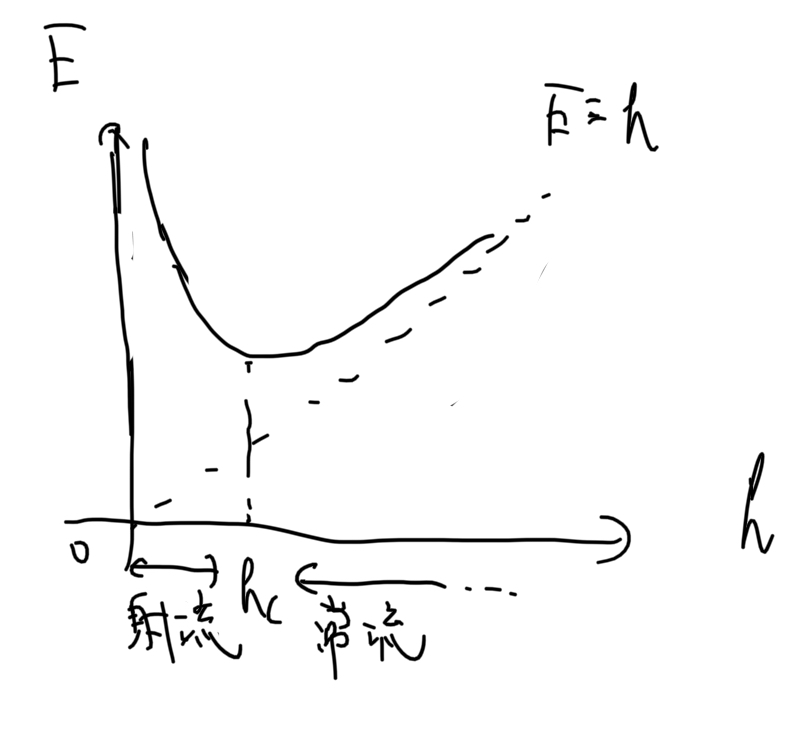
\includegraphics[width=0.3\hsize]{fig1.png}
  \caption{比エネルギー$E$と水深$h$の関係}
\end{figure}

\subsection{}
跳水前後の断面をそれぞれ断面1,断面2とする。これらの断面の間で運動量保存則
\begin{equation}
  \rho q (v_2 - v_1) 
  = \frac{1}{2} \rho g h_1^2 - \frac{1}{2} \rho g h_2^2
\end{equation}
が成り立つ。$v_1 = q / h_1, v_2 = q / h_2$を代入し整理すると、
\begin{equation}
  q = \sqrt{\frac{1}{2} g h_1 h_2 (h_1 + h_2)}
\end{equation}
となる。$h_1 = 0.2 \mathrm{m}, h_2 = 0.8 \mathrm{m}, g = 9.8 \mathrm{m/s^2}$を代入すると、
$q = 0.89 \mathrm{m^2/s}$である。この$q$を用いて、
\begin{equation}
  \Delta E = \left(\frac{q}{2g h_1^2} + h_1\right)
  - \left(\frac{q}{2g h_2^2} + h_2\right) = 0.33 \mathrm{m}
\end{equation}
を得る。

\subsection{}
地球を球であると思えば、地球の半径を$R$として図2のように、$y = R (\varphi - \varphi_0)$、
すなわち、$\varphi = y / R + \varphi_0$の関係が成り立つ。\par
\begin{figure}[htb]
  \centering
  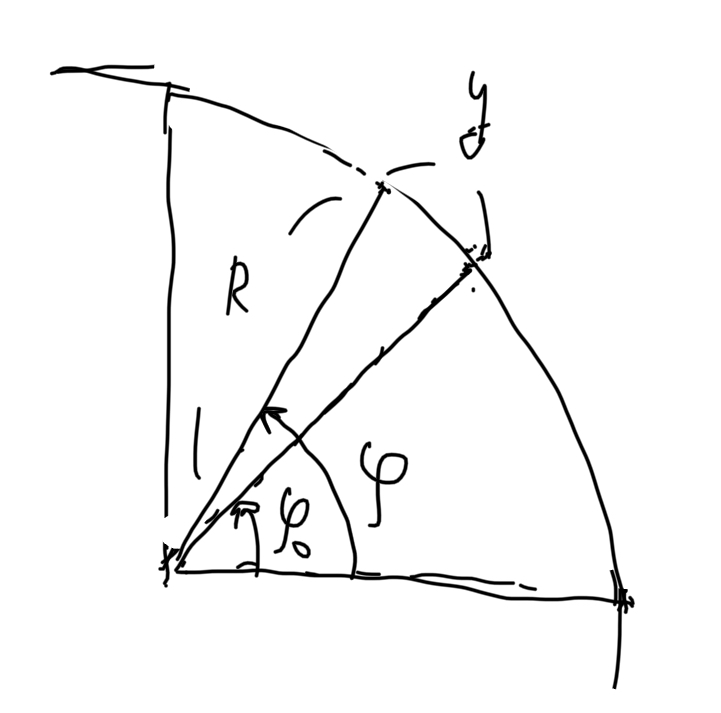
\includegraphics[width=0.3\hsize]{fig2.png}
  \caption{$y$と$\phi$の関係}
\end{figure}
$f$を$y = 0$の近傍で1次近似すると、
\begin{equation}
  f \simeq f_0 + \left.\frac{\partial f}{\partial y}\right|_{y=0} y
\end{equation}
であるから、
\begin{equation}
  \beta = \left.\frac{\partial f}{\partial y}\right|_{y=0}
  = \left.\frac{\mathrm{d} f}{\mathrm{d} \varphi}\right|_{\varphi = \varphi_0}
  \left.\frac{\mathrm{d} \varphi}{\mathrm{d} y}\right|_{y=0} 
  =\frac{2 \Omega \cos \varphi_0}{R}
\end{equation}
となる。数値を代入すると、
\begin{equation}
  \beta = \frac{2 \times \frac{2 \pi}{24 \times 3600} \times 0.71}{6.4 \times 10^6} = 1.6 \times 10^{-11}
\end{equation}
を得る。

\subsection{}
限界流では、$R_F = 1$より、$12 u = \beta a^2$である。したがって、
\begin{equation}
  a = \sqrt{\frac{12 u}{\beta}} = \sqrt{\frac{12 \times 12}{1.6 \times 10^{-11}}}
  = 3 \times 10^6 \mathrm{m}
\end{equation}
となる。

\subsection{}
ジェット気流の幅の増加に伴って渦が発生し、流れが蛇行する。\par
渦は一度発生すると渦度の保存によってなかなか消滅せず、ブロッキング現象の起こった状態の気象状態が持続する。
ここに高気圧が停滞すれば乾燥天候の持続により干ばつが引き起こされ、相補的に停滞性のある低気圧が位置すれば降水が長期間続く。
干ばつの社会的影響としては、水不足と農作物被害が挙げられる。大雨の社会的影響として、河川流量の増加に伴い水害が引き起こされる危険がある。

\section{}
\subsection{}
流れが管軸方向に一様であるから$\frac{\partial u_z}{\partial z} = 0$、
また、管軸まわりに対象であるから、$\frac{\partial u_{\theta}}{\partial \theta} = 0$
が成り立つ。
これを連続式に代入すると、
\begin{equation}
  \frac{\partial u_r}{\partial r} + \frac{u_r}{r} = 0
\end{equation}
となる。$u_r = 1/r$とかこれ満たしますけどね、、
\end{document}